%
%  --- USU thesis and dissertation template ---
%
% Time-stamp: "[thesis.tex] last modified by Scott Budge (scott) on 2022-04-26 (Tuesday, 26 April 2022) at 11:43:40 on goga"
%
%  Modified to use the new usuthesis.cls by Allan McInnes
%
%  Specify department ('ee' or 'ce' or 'me' or 'ae' or 'cee') and document type ('msthesis',
%  'msreport', or 'dissertation') in the documentclass options. 
%
%  Including the 'proposal' option will generate a proposal for a thesis
%  or dissertation, rather than a final document (this mostly just 
%  alters the cover page).
%
%  See the opening comments of usuthesis.cls for more information on 
%  available options
%
%  To create finished document run:
%    latex thesis.tex
%    bibtex thesis (or sample-chapter1, etc., if using multiple-paper format)
%    latex thesis.tex
%    latex thesis.tex
%
%  Info: $Id: thesis.tex 1183 2021-06-28 16:49:30Z scott $   USU
%  Revision: $Rev: 1183 $
% $LastChangedDate: 2021-06-28 10:49:30 -0600 (Mon, 28 Jun 2021) $
% $LastChangedBy: scott $
%

% For the ECE Department:
%\documentclass[ee,msthesis]{usuthesis}
%\documentclass[ce,msthesis]{usuthesis}
\documentclass[ee,dissertation]{usuthesis}
%\documentclass[ee,proposal]{usuthesis}
%\documentclass[ce,dissertation]{usuthesis}
% For the MAE Department:
%\documentclass[me,msthesis]{usuthesis}
%\documentclass[ae,msthesis]{usuthesis}
%\documentclass[me,dissertation]{usuthesis}
%\documentclass[ae,dissertation]{usuthesis}
% For the CEE Department:
%\documentclass[cee,msthesis]{usuthesis}
%\documentclass[cee,dissertation]{usuthesis}


%{{{ Packages
\usepackage{amssymb}           % add ams symbols stuff
\usepackage{graphicx}          % add graphics
\usepackage{subcaption}
\usepackage{url}
%\usepackage{flafter}           % Cause floats to appear after
                               % environment.
%\usepackage{siunitx}           % Provides standard formatting of SI units.
\usepackage{listings}          % Use when including computer code.


% Include TikZ and PGF packages for high-quality graphics, schematics
% and plots. This is optional; at the current time, when run with
% latex to create a .dvi file, the xdvi viewer will produce incorrect
% formatting for the TikZ figures.  If the .dvi file is converted to
% pdf using "dvipdf" the resulting pdf file is correct.  If this
% example is used with  pdflatex, the resulting TikZ figures in the
% output look fine.
\usepackage{tikz}       		% The base tikz+pgf package
\usetikzlibrary{arrows,shapes}	% Optional tikz extensions
\usepackage[american]{circuitikz}	% TikZ-based package for schematic drawings
\usepackage{pgfplots}			% Tikz-based package for making plots 
\pgfplotsset{compat=1.6}        % This *might* be necessary for your
                                % version of pgfplots.

\usepackage{hyperref} % Creates hyperlinks within document
\hypersetup{colorlinks=true, linkcolor=blue,
  citecolor=blue,urlcolor=blue} % Use when compiling the digital copy
% \hypersetup{colorlinks=true, linkcolor=black,
% citecolor=black,urlcolor=black} % Use when compiling the printed copy

% The following allows for hyperlinked DOIs to be inserted in the
% manuscript by using \doi{}.
\usepackage{doi}

% Set spacing around figures and tables to triple space
\setlength{\intextsep}{2em} % Vertical space above & below [h] floats
\setlength{\textfloatsep}{2em} % Vertical space below (above) [t] ([b]) floats

% The following is added if you are using the multiple-paper format to
% add references after each chapter:
%\usepackage[sectionbib]{chapterbib}

%}}}

% Author and Title Information
\author{John Q. Engineer}
\title{A Complicated and Impressive Sounding Title that is Too Long
  For a Single Line While Including Everything}

% The Committee
\majorprof{Richard P. Feynmann, Ph.D.}
\firstreader{Robert L. Forward, Ph.D.}
\secondreader{Albert Einstein, Ph.D.}
\thirdreader{Gottfried Liebniz, Ph.D.}
\fourthreader{Isaac Newton, Ph.D.}

% Graduate Dean
\graddean{ D. Richard Cutler, Ph.D.}
\deantitle{ Vice Provost of Graduate Studies}

% Degree Information
%\degree{Master of Science}
\degree{Doctor of Philosophy}
\month{May}
\gradyear{2022}

\begin{document}
    %{{{ Frontmatter
    \preliminaries   % set frontmatter style
    
    \maketitle
    \makecopyright        % optional
    
    %
%

\begin{abstract}
% A space is needed before the text starts so that the first paragraph
% is indented properly. Max 350 words.

    Illness, injury, and other impediments are common occurrences of every day life.
    Such impediments prevent or deter agents from participating in important parts
    of the voting process, in particular deliberation, bargaining, and the voting
    itself.
    Without participation, the results of the vote may change.
    There is a need to provide a mechanism by which agents are still able to
    participate in such processes to ensure their vote is represented.
    We examine single-vote/single-winner
    % 05/05/2023: \vicki{Explain unified-vote}
    % Replaced with "single vote," since explaining "unified vote" would probably
    % make may abstract too long.
    proxy voting in a one-dimension continuous
    preference space using a combination of $L_p$ aggregation methods.
    As part of this examination, we develop and examine `coordination mechanisms,' by
    which proxies and their constituents are able to find a way to combine their
    preferences in order for constituents to still have their voices heard.
    In exchange, their proxy gains more weight and is able to have a stronger voice in
    deliberations.
    We employ a continuous preference space model and determine the result of a vote
    as a point in the model's space.
    This model allows for more options than the vote only passing or failing by
    allowing the outcome to directly correlate to actions to be taken, such as the
    amount of money to spend.
    Such an ability increases the granularity of the results and allows us to
    better determine how much error is introduced by proxy voting.
    The continuous preference space model also provides a more expressive way of
    casting a vote.
    We show that proxy voting is effective in many scenarios, and that it is
    consistently better than not allowing inactive agents to vote.


\end{abstract}


% Local Variables:
% TeX-master: "newhead"
% End:

    %
%  Time-stamp: "[publicabstract.tex] last modified by Scott Budge (scott) on
%  2011-08-09 (Tuesday, 9 August 2011) at 09:17:43 on goga"
%
%  Info: $Id$   USU
%  Revision: $Rev$
% $LastChangedDate$
% $LastChangedBy$
%

\begin{publicabstract}
% A space is needed before the text starts so that the first paragraph
% is indented properly.

    % TODO: Rewrite

\end{publicabstract}


% Local Variables:
% TeX-master: "newhead"
% End:

    %
% Dedication
%

\begin{dedication}
% \begin{center}
    To Danielle, my constant companion and eternal partner.
    
    You are my light and my star, my guiding hope.
    I love you.
\newline
\newline

    And to Miriam, who joined us in our adventure.
    
    May you lift others up and help them to be as brilliant as you.
% \end{center}
% 
% If you intend to have a dedication longer than one line, do not put
% it in a centering environment.  It will look better.
\end{dedication}
  % optional 
    %
% This is an example of an acknowledgements page.  This is optional,
% and can contain anything you want to say.
%
%
%  Time-stamp: "[acknowl.tex] last modified by Scott Budge (scott) on 2011-08-08 (Monday, 8 August 2011) at 15:45:15 on goga"
%
%  Info: $Id$   USU
%  Revision: $Rev$
% $LastChangedDate$
% $LastChangedBy$
%

\begin{acknowledgments} 
I am so happy that my advisor helped me.....
\\
\begin{flushright} 
John Q. Engineer 
\end{flushright}
\end{acknowledgments}

     % optional
    
    \tableofcontents 
    \listoftables 
    \listoffigures
    
%    %
% Contains notations used in this paper.
% Mostly used because I hate having to search throughout a paper to figure
% out what a symbol means in a math equation.
%
%! suppress = EscapeAmpersand
\newcommand{\notationheader}[1]{\multicolumn{2}{l}{\textbf{#1}}\\}
\newcommand{\notationdesc}[2]{#1 & #2\\}

\begin{notation}
\setlength{\tabcolsep}{3mm}{
    % TODO: Alphabetize these by symbol
    \begin{tabular}{ll}
        \notationheader{Equations}
        \notationdesc{\agent}{An individual agent}
        \notationdesc{\agents}{The set of all agents}
        \notationdesc{\cost}{Cost}
        \notationdesc{\loss}{Loss}
        \notationdesc{\real}{The set of all real numbers}
        \notationdesc{\system}{A system}
        \notationdesc{\systemspace}{The space within a system operates}
        \notationdesc{\truth}{Truth}
        \notationdesc{\agenttruth}{The truth as estimated by an agent}
        \notationdesc{\systemagents}{The agents of a system}
        \notationdesc{\systemcost}{The cost of a system}
        \notationdesc{\systemloss}{The loss of a system}
        \notationdesc{\systemtruth}{The truth as estimated by a system}
    \end{tabular}
}

% The table as defined above will fill one page. If you need more room to list
% notation you will need to create a second table, and place it below this 
% comment. This new table will appear one a new page.

\end{notation}

  % optional
    %
% This is an example of an acronyms page.  
% Acronyms are laid out in tabular format.
%
%  Time-stamp: "[acronyms.tex] last modified by Scott Budge (scott) on 2011-08-08 (Monday, 8 August 2011) at 15:45:41 on goga"
%
%  Info: $Id$   USU
%  Revision: $Rev$
% $LastChangedDate$
% $LastChangedBy$
%

\begin{acronyms}

% \renewcommand{\arraystretch}{1.5}
% \setlength{\tabcolsep}{3mm}
% {\begin {tabular}{ll}
% BFCS & body-fixed coordinate system\\
% CEF   &composite energy function (related to ILC)\\
% CSOIS &Center for Self-Organizing and Intelligent Systems\\
% CV    &certainty value (related to HIMM)\\
% DOF   &degree of freedom\\
% EKF   &extended Kalman filter\\
% FOG   &fiber optic gyro\\
% FOV &field of view of a camera\\
% GAIC &geometric Akaike information criterion\\
% GMDL &geometric minimum description length criterion\\
% GRO &growth rate operator (related to HIMM)\\
% HIMM &histogram in-motion mapping\\
% HOSA &higher-order spectral analysis (related to Matlab toolbox)\\
% IBO &identifier-based observer (related to PDS)\\
% IIC &identical initial condition (related to ILC)\\
% ILC &iterative learning control\\
% ICS &inertial coordinate system\\
% LAO &linear approximation-based observer (related to PDS)\\
% LQG &linear quadratic Gaussian\\
% LS &least squares\\
% LTV &linear time-varying\\
% NN &neural network\\
% OCS &obstacle cluster strength (related to HIMM)\\
% ODIS &omni-directional inspection system, a robot at the CSOIS center\\
% ODV &omni-directional vehicle\\
% \end {tabular}}

\end{acronyms}
  % optional  
    %}}}
    %{{{ The main body of the thesis
    \body  % set main body style
    % Chapters
    %
%  This is an example of how a LaTeX thesis should be formatted.  This
%  document contains chapter 1 of the thesis.
%
%  Time-stamp: "[sample-chapter1.tex] last modified by Scott Budge (scott) on 2017-01-12 (Thursday, 12 January 2017) at 10:20:50 on goga.ece.usu.edu"
%
%  Info: $Id: sample-chapter1.tex 998 2017-03-21 16:44:33Z scott $   USU
%  Revision: $Rev: 998 $
% $LastChangedDate: 2017-03-21 10:44:33 -0600 (Tue, 21 Mar 2017) $
% $LastChangedBy: scott $
%

\chapter{INTRODUCTION}
%%%%%%%% This line gets rid of page number on first page of text
\thispagestyle{empty}
%%%%%%%%%%%%%

Image compression or image coding is the process of reducing the
redundancy in the image data that may result in some loss of
information.  Vector quantization (VQ)\footnote{The acronym VQ is used
  as an abbreviation for both vector quantization and vector
  quantizer.} is one such technique.

\section{Background}
Binary splitting is illustrated in Fig.~\ref{fig:split}.

\begin{figure}[htbp]
\centering
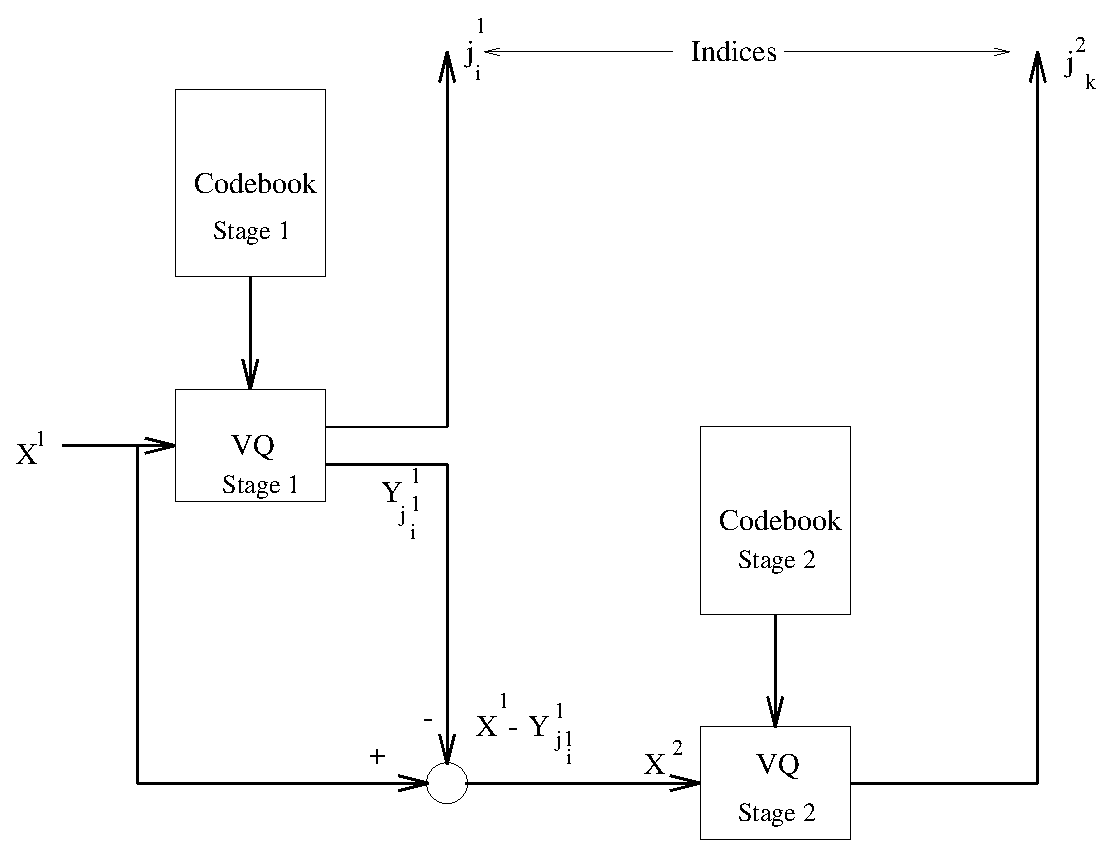
\includegraphics[width=0.7\textwidth]{samplefig}
\caption{Binary splitting.}
\label{fig:split}
\end{figure}
This figure is generated using an open-source figure drawing package
(called {\tt fig}).  Any figure drawing package can be used to
generate figures.  The easiest format for output is to output the
figures in {\tt .pdf} format for inclusion in the {\tt .tex} file.

% For the following three examples, note the problems with the xdvi
% viewer described in the thesis.tex and the README.txt files.

%%%%%%%%%%%%%%%%%%%%%%%%%%%%%%%%%%%%%%%%%%%%%%%%%%%%%%%%%%%%%%%%%%
% TikZ example:  This is the same as the above figure, except done
% using TikZ.
%%%%%%%%%%%%%%%%%%%%%%%%%%%%%%%%%%%%%%%%%%%%%%%%%%%%%%%%%%%%%%%%%%
\begin{figure}[!t]
	\begin{center}
		\begin{tikzpicture}[every text node part/.style={align=center}]
			% Place nodes:
			\draw (0,0) node[draw] (book1) {{\em Codebook}\\ {\small Stage 1}};
			\draw ($(book1) + (0,-2)$) node[draw] (vq1) {{\em VQ}\\ {\small Stage 1}};
			\draw ($(vq1) + (3,-3)$) node[circle,draw,minimum height=1cm] (adder) {$\Sigma$};
			\draw ($(adder) + (5,0)$) node[draw] (vq2) {{\em VQ}\\ {\small Stage 2}};
			\draw ($(vq2) + (0,2)$) node[draw] (book2) {{\em Codebook}\\ {\small Stage 2}};
			
			% Draw arrows:
			\draw [-latex] (book1.south) -- (vq1.north);
			\draw [-latex] (book2.south) -- (vq2.north);
			\draw [-latex] ($(vq1.north east)+(0,-.25)$) node(vqout1) {} -| ($(adder.north)+(0,6)$) node[anchor=south west] (ji) {$j_i$};
			\draw [-latex] ($(vq1.south east)+(0,.25)$) node(vqout2) {} -| (adder.north);
			\draw [-latex] (vq1.west) -- ($(vq1.west)+(-1,0)$) node (in) {} |- (adder.west);
			\draw [-latex] (vq2.east) -| ($(ji.south west) + (7,0)$) node[anchor=south west] (jk2) {$j_k^2$};
			\draw ($(vq1.west)+(-2,0)$) node[anchor=east] {$X^1$} to[short,o-*] (in);
			\draw [-latex] (in) -- (vq1.west);
			\draw [-latex] (adder.east) -- (vq2.west);
			
			% Draw remaining labels:
			\draw (vqout2) node[anchor=north west] {$Y_{j_i^1}^1$};
			\draw (adder.north) node[anchor=south east] {$-$};
			\draw (adder.west) node[anchor=south east] {$+$};
			\draw (adder.east) node[anchor=south west] {$X^1-Y_{j_i^1}^1$};
			\draw (vq2.west) node[anchor=south east] {$X^2$};
			
			% Draw annotation:
			\draw ($(ji)!0.5!(jk2) + (0,1)$) node (indices) {\Large Indices};
			\draw[thick,-triangle 45] (indices.west) to [out=180,in=45] (ji.north east);
			\draw[thick,-triangle 45] (indices.east) to [out=0,in=135] (jk2.north west);
		\end{tikzpicture}
		\caption{Binary splitting (drawn with TikZ).}
		\label{fig:split_tikz}
	\end{center}
\end{figure}

%%%%%%%%%%%%%%%%%
% CircuiTikZ example:
%%%%%%%%%%%%%%%%%
\begin{figure}[!t]
	\begin{center}
		\begin{tikzpicture}
			\draw (0,0) node[op amp,scale=0.75] (oa){};
			\draw (oa.out) to[short, -*] ++(1,0) node (n1) {};
			\draw (n1.base) -- ++(1,0) to[C,l^=$C_S$,v_=$V_{\textrm{\small out,ofs}}$] ++(3,0) 	node[anchor=west] (n4) {$V_{\textrm{\small out}}$};
			\draw (oa.-) to[short,-*] ++(-1,0) node (n2) {};
			\draw (n2.base) |- ++(1,2) to[C] ++(2,0) -| (n1.base);
			\draw ($(oa.+)+(0,-3)$) node[ground] {}  to[vsource=$V_{\textrm{\small in,ofs}}$] (oa.+);
			\draw (n2.base) to[C] ++(-2,0) node[anchor=east] (n3) {$V_{\textrm{\small in}}$};
		\end{tikzpicture}
		\caption{Circuit example drawn using circuitikz.}
		\label{fig:circuitikz_exmple}
	\end{center}
\end{figure}

There are many other ways to create figures.  One package compatible
with \LaTeX\ is TikZ.  An example is given in
Fig.~\ref{fig:split_tikz}. This is identical to Fig.~\ref{fig:split},
except that it is done within the compiling process of \LaTeX.
Another example of a third-party figure package is given in
Fig.~\ref{fig:circuitikz_exmple}.  This circuit was generated using
the {\tt circuitikz} package.

It is important that there is no text between figures when they are
referenced close together in the text.  They should be ``stacked''
without text in between as seen above.

A final way of creating graphs is to use a open-sourse package called
{\tt PGFPlots}.  An example of a good-looking graph generated using
this package is given in Fig~\ref{fig:pgfplots_example}.  Note that
this figure is large enough that it is pushed by \LaTeX\ to another
page by itself and nicely centered.
%%%%%%%%%%%%%%%%%
% PGFplots example:
%%%%%%%%%%%%%%%%%
\begin{figure}[tbh]
\begin{center}
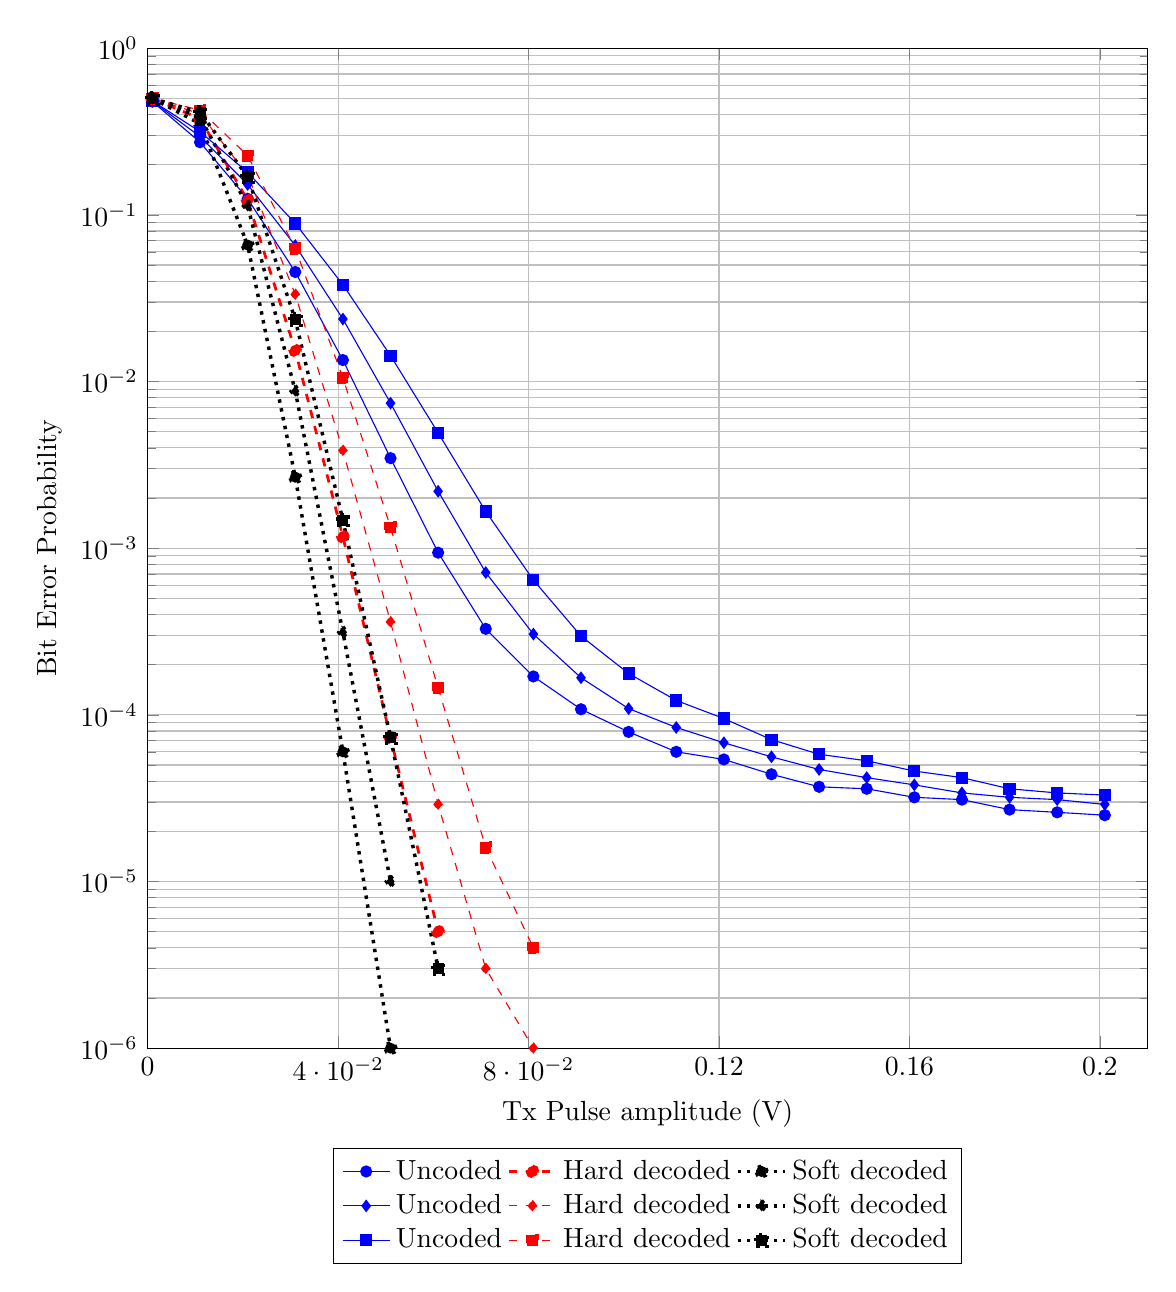
\begin{tikzpicture}
\begin{semilogyaxis}
[% 
scale only axis, 
width=5in, 
height=5in, 
xmin=0, 
xmax=0.21, 
xtick={0, 0.04, ..., 0.2},
ymin=1e-006, 
ymax=1, 
yminorticks=true, 
%xlabel={$\text{Tx Pulse amplitude }(\si{\volt})$},
xlabel={Tx Pulse amplitude (V)},
ylabel={Bit Error Probability}, 
xmajorgrids, 
ymajorgrids, 
yminorgrids,
legend columns=3,
legend style={at={(0.5,-0.1)},anchor=north},%{at={(0.5,-0.5)},anchor=south},
cycle multi list={%
   color list\nextlist
   [3 of]mark list}
]

%%%%%%%%%%%%%%%%%%%%%%%%%%%%%%%%%%%%%%%%%%%%%%%%%%%%%%%%%%%%%%%%%%
%8p_NF4_uncoded
\addplot [ color=blue, solid, mark=*, mark options={fill=blue} ] 
coordinates{  
(0.001,0.478052)(0.011,0.272706)(0.021,0.124776)(0.031,0.045402)(0.041,0.013449)(0.051,0.003469)(0.061,0.00094)(0.071,0.000328)(0.081,0.00017)(0.091,0.000108)(0.101,7.9e-005)(0.111,6e-005)(0.121,5.4e-005)(0.131,4.4e-005)(0.141,3.7e-005)(0.151,3.6e-005)(0.161,3.2e-005)(0.171,3.1e-005)(0.181,2.7e-005)(0.191,2.6e-005)(0.201,2.5e-005)  
    };
\addlegendentry{Uncoded}

%8p_NF4_hard
\addplot [ color=red, line width=1pt,dashed, mark=*,  mark options={fill=red},]
coordinates{  
(0.001,0.499268)(0.011,0.377753)(0.021,0.122226)(0.031,0.01535)(0.041,0.001172)(0.051,7.3e-005)(0.061,5e-006)(0.071,0)  
};
\addlegendentry{Hard decoded}

%8p_NF4_soft
\addplot [ color=black, dotted, line width=1.25pt,mark=*, mark options={fill=black} ] 
coordinates{  (0.001,0.49911)(0.011,0.352208)(0.021,0.065849)(0.031,0.002668)(0.041,6e-005)(0.051,1e-006)  
};
\addlegendentry{Soft decoded}

%%%%%%%%%%%%%%%%%%%%%%%%%%%%%%%%%%%%%%%%%%%%%%%%%%%%%%%%%%%%%%%

%%%%%%%%%%%%%%%%%%%%%%%%%%%%%%%%%%%%%%%%%%%%%%%%%%%%%%%%%%%%%%%%%%
%8p_NF5_uncoded
\addplot [ color=blue, solid, mark=diamond*, mark options={fill=blue} ]
coordinates{  (0.001,0.480507)(0.011,0.294723)(0.021,0.1521)(0.031,0.065413)(0.041,0.023695)(0.051,0.007415)(0.061,0.002195)(0.071,0.000714)(0.081,0.000305)(0.091,0.000167)(0.101,0.000109)(0.111,8.4e-005)(0.121,6.8e-005)(0.131,5.6e-005)(0.141,4.7e-005)(0.151,4.2e-005)(0.161,3.8e-005)(0.171,3.4e-005)(0.181,3.2e-005)(0.191,3.1e-005)(0.201,2.9e-005)      };
\addlegendentry{Uncoded}

%8p_NF5_hard
\addplot [ color=red, dashed, mark=diamond*, mark options={fill=red} ]
coordinates{  (0.001,0.499279)(0.011,0.403647)(0.021,0.17325)(0.031,0.033326)(0.041,0.003852)(0.051,0.000361)(0.061,2.9e-005)(0.071,3e-006)(0.081,1e-006)        
};
\addlegendentry{Hard decoded}

%8p_NF5_soft
\addplot [ color=black, dotted, line width=1.25pt,mark=diamond*, mark options={fill=black} ]
coordinates{  (0.001,0.499265)(0.011,0.385162)(0.021,0.113072)(0.031,0.008749)(0.041,0.000313)(0.051,1e-005)(0.061,0)  
};
\addlegendentry{Soft decoded}
%%%%%%%%%%%%%%%%%%%%%%%%%%%%%%%%%%%%%%%%%%%%%%%%%%%%%%%%%%%%%%%

%%%%%%%%%%%%%%%%%%%%%%%%%%%%%%%%%%%%%%%%%%%%%%%%%%%%%%%%%%%%%%%%%%
%8p_NF6_uncoded
\addplot [ color=blue, solid, mark=square*, mark options={fill=blue} ]
coordinates{  (0.001,0.482503)(0.011,0.315407)(0.021,0.179759)(0.031,0.088806)(0.041,0.038068)(0.051,0.014303)(0.061,0.004914)(0.071,0.001661)(0.081,0.000644)(0.091,0.000297)(0.101,0.000177)(0.111,0.000122)(0.121,9.5e-005)(0.131,7.1e-005)(0.141,5.8e-005)(0.151,5.3e-005)(0.161,4.6e-005)(0.171,4.2e-005)(0.181,3.6e-005)(0.191,3.4e-005)(0.201,3.3e-005)       };
\addlegendentry{Uncoded}

%8p_NF6_hard
\addplot [ color=red, dashed, mark=square*, mark options={fill=red} ]
coordinates{
(0.001,0.499326)(0.011,0.424875)(0.021,0.22663)(0.031,0.062807)(0.041,0.010536)(0.051,0.001333)(0.061,0.000145)(0.071,1.6e-005)(0.081,4e-006)(0.091,0)  
};
\addlegendentry{Hard decoded}

%8p_NF6_soft
\addplot [ color=black, dotted, line width=1.25pt,mark=square*, mark options={fill=black} ] 
coordinates{  (0.001,0.499363)(0.011,0.411563)(0.021,0.169253)(0.031,0.02352)(0.041,0.001472)(0.051,7.3e-005)(0.061,3e-006)(0.071,0)      
};
\addlegendentry{Soft decoded}

%%%%%%%%%%%%%%%%%%%%%%%%%%%%%%%%%%%%%%%%%%%%%%%%%%%%%%%%%%%%%%%

\end{semilogyaxis}

\end{tikzpicture}

\caption{Example figure made with PGFplots. Originally created in Matlab, then exported using the Matlab2TikZ script (available from Matlab Central). Then pasted into the \LaTeX\ document and edited for style. \label{fig:pgfplots_example} }
\end{center}
\end{figure}



% For use with multiple-paper format, uncomment the fillowing:
% \pagebreak
% \bibliographystyle{IEEEtran}
% \bibliography{IEEEabrv,BibFile1}  % uses the references stored in BibFile1.bib for this chapter

% Local Variables:
% TeX-master: "newhead"
% End:

    %
%  This is an example of how a LaTeX thesis should be formatted.  This
%  document contains chapter 2 of the thesis.
%
%  Time-stamp: "[sample-chapter2.tex] last modified by Scott Budge (scott) on 2016-07-28 (Thursday, 28 July 2016) at 08:40:50 on goga.ece.usu.edu"
%
%  Info: $Id: sample-chapter2.tex 967 2016-07-28 15:33:29Z scott $   USU
%  Revision: $Rev: 967 $
% $LastChangedDate: 2016-07-28 09:33:29 -0600 (Thu, 28 Jul 2016) $
% $LastChangedBy: scott $
%

\chapter{RESIDUAL VECTOR QUANTIZATION AND ITS PROBLEMS}

\section{Residual Vector Quantization (RVQ)}

A $P$-stage RVQ consists of a sequence of $P$ single stage Vector
Quantizers.  Let us assume that the RVQ is made up of ESVQ stages.
Each ESVQ is fully described by the set \{ $A^{\rho}, Q^{\rho},
P^{\rho}$ \}.  The method for designing the ESVQ is given in
Algorithm~\ref{alg:LBG}.  Note that this is the ``usual'' codebook
design algorithm.% Note how quotes are used in the previous sentence.

%This is HOW SECTION HEADINGS EXCEEDING 3 inches should be declared
%so that it wraps in the heading but not in the TOC.
%\section[Reasons for the Poor Performance of RVQs]{Reasons for the
%  Poor \newline Performance of RVQs}

%Normally you do the following, and ignore the 3-inch rule:
Throw in some citations \cite{shucker,tbrady,moon,bar1}.


\begin{alg}
\begin{tabbing}
{\bf Input:} \=  \\ 
    \> Training vectors ($V_t$), \\
    \> Distortion measurement rule $d$, \\
    \> Codebook size $N$, \\
    \> Threshold $\varepsilon$ \\
{\bf Output: } \\
 \> Codebook Vectors, $Cb_i$  \\
{\bf Begin} \\
 \> Select $N$ initial codevectors, $Cb_i$  \\
 \> {\bf Do} \= \\
 \> \> {\bf Begin} \= \\
 \> \> \> Partition $V_t$ \\
 \> \> \> $Dist_{prev} = Dist_{current}$ \hspace{1.2in}\=/* Dist is the average */ \\
 \> \> \> Calculate $Dist_{current}$ \> /* distortion of all the */ \\
 \> \> \> Calculate Centroids of $N$ groups of $V_t$ \> /* training vectors when */\\
 \> \> \> $Cb_i$ = Centroid of that group \> /* partitioned or encoded */ \\
 \> \> {\bf End} \\
 \> {\bf while} $\{(Dist_{prev} - Dist_{current})/Dist_{prev} \geq \varepsilon\}$ \\
{\bf End} \\
\end{tabbing}
\caption{LBG}
\label{alg:LBG}
\end{alg}

\section{Reasons for the Poor Performance of RVQs}

\begin{equation}
d(X^{\rho},Y_i^{\rho} + A^{\rho+1}+ \cdots + A^{P}) \leq d(X^{\rho},A^{\rho} + A^{{\rho}+1} + \cdots + A^P)
\label{cond-optpart}
\end{equation}

It can be noticed from the above equation that while the traditional
RVQ partitions are based on the stagewise residues, the optimal RVQ
partitions are based on the final residues. As is evident from
(\ref{cond-optpart}), the optimal codevectors are unique.  The
equivalent codevectors are obtained by summing all possible
combinations of the codevectors of all stages.  These represent the
set of reconstruction vectors possible at the decoder.

\section{Methods to Improve RVQ Performance}

The various  methods either suboptimal or optimal used in codebook generation
 and in the quantizer (RVQ) implementation are dealt with here.  The common
 goal of all these methods is to improve the performance of the RVQ. 

\subsection{Brute Force RVQ or Stagewise RVQ (SRVQ)}

The new codevectors are obtained by adding the centroids of the
stagewise residues to the old codevectors.  This can be done using a
random splitting technique or a selective splitting technique.

\subsection{Exhaustive Search RVQ (ESRVQ)}

ESRVQ is the optimal RVQ described in the previous section.  ESRVQ, as
the name suggests, exhaustively searches all the {\em equivalent}
codevectors as shown in (\ref{cond-optpart}).  Centroids of the final
residues are added to the codevectors during each iteration of the
codebook design, to obtain the new optimal codevectors for the given
partition.

\subsection{Deep Search RVQ}

Although ESRVQ is optimal, it needs an exhaustive search encoder. We
must be able to create the encoder using an optimal method. 


\subsection{Comparison of SRVQ, DSRVQ, and ESRVQ Encoders}

This section compares the different encoders presented previously.
The different encoders have different performance and complexity, and
so must be compared using a common basis.  This is difficult to do,
since we must first establish the criteria we will use.

\subsection{Algorithm for Generating Jointly Optimized
Codebooks}


The ESRVQ is not instrumentable and the DSRVQ does not use a
tree-structured encoder.  Hence Barnes et al. proposed the reflection
symmetric RVQ or the rRVQ~\cite{Barn-JORVQ}.  The rRVQ uses a
tree-structured encoder similar to SRVQ although it differs from the
traditional RVQ or the SRVQ encoder in that it is slightly more
complex.  The rRVQ codebook is also more structured than the
traditional RVQ.

Some other citations are in
\cite{moon,BAK-nonadVQ,B-JORVQ,Barnes-RQ,Datasheet1,CID-example,Privatecom,Patent1,Berg-RD,CMH}.

\subsection{Reflection Symmetric RVQ (rRVQ)}

The ESRVQ is not instrumentable and the DSRVQ does not use a
tree-structured encoder.  Hence Barnes et al. proposed the reflection
symmetric RVQ or the rRVQ~\cite{Barn-JORVQ}.  The rRVQ uses a
tree-structured encoder similar to SRVQ although it differs from the
traditional RVQ or the SRVQ encoder in that it is slightly more
complex.  The rRVQ codebook is also more structured than the
traditional RVQ.

The structured nature of the rRVQ codebook allows for a reduction of
the complexity of the the implementation.

\subsubsection{Binary rRVQ}

It was already stated that for the optimal performance of the RVQ, an
exhaustive search encoder must be used. To avoid this in rRVQ the
codebook is constrained in such a way that the nearest neighbor
stagewise equivalence classes are simply connected and
convex~\cite{Barn-JORVQ}.  A reflection symmetry is forced between the
stagewise codevectors of the binary rRVQ to obviate the suboptimality
caused by {\em entanglement} and {\em overlapping} discussed in the
previous chapter.  Barnes et al. derived the optimality conditions
for the rRVQ quantitatively~\cite{Barn-JORVQ}.  They stated their
results as follows~\cite[pp. 3--4]{Barn-JORVQ}:
\begin{quotation}
\begin{spacing}{1}
  ``The difficulty in achieving optimality is that it is difficult.  We
  observed that it was necessary to look at the conditions for
  optimality before we could proceed.  We then proceeded with caution.

  Having proceeded, we applied the conditions for optimality.  To our
  amazement, we found our results were optimal.''
\end{spacing}
\end{quotation}


\subsection {Distortion Results and Analysis}
Table \ref{table:dist4x4} gives the PSNR in dB of the reconstructed test image,
compressed (encoded and decoded) using the codebooks generated by SRVQ. 

\begin{table}[!t] % table at top of page.
  % increase table row spacing, adjust to taste
  \renewcommand{\arraystretch}{1.3}
  \caption{Performance results of ESRVQ, rRVQ, SRVQ, and DSRVQ of 4x4
    vectors (PSNR~in~dB).}
  \label{table:dist4x4}

  \centering
  \begin{tabular}{||c|c||c|c||c|c||c|c||c|c||} \hline
    No. of  & &
    \multicolumn{2}{c||}{SRVQ} & \multicolumn{2}{c||}{DSRVQ} &
    \multicolumn{2}{c||}{ESRVQ} & \multicolumn{2}{c||}{rRVQ} \\ \cline{3-10}
    Stages & bps & Unopt & JO & Initial & JO & Initial & JO & Initial & JO \\ \hline
  \end{tabular}
\end{table}

The ESRVQ is not instrumentable and the DSRVQ does not use a
tree-structured encoder.  Hence Barnes et al. proposed the reflection
symmetric RVQ or the rRVQ~\cite{Barn-JORVQ}.  The rRVQ uses a
tree-structured encoder similar to SRVQ although it differs from the
traditional RVQ or the SRVQ encoder in that it is slightly more
complex.  The rRVQ codebook is also more structured than the
traditional RVQ.

It is important to recognize at this point, that rRVQ is a suboptimal
method for covering the vector space.  It is therefore important to
make sure that the best possible vectors are chosen for the codebook.

% For use with multiple-paper format, uncomment the fillowing:
% \pagebreak
% \bibliographystyle{IEEEtran}
% \bibliography{IEEEabrv,BibFile2}  % uses the references stored in BibFile2.bib for this chapter

% Local Variables:
% TeX-master: "newhead"
% End:

    
    % Endmatter
    % For BibTeX references: specify a .bib file and a style.
    % The style used here is for IEEE transactions formatting:
    \references{IEEEabrv,sample}{IEEEtran}
    % The style used here is for AIAA formatting:
%    \references{IEEEabrv,sample}{aiaa}
    
    %
%  Example Appendix pages.
%  Modified to use new usu-thesis-mk2 appendix facilities.
%
%  Time-stamp: "[appendix.tex] last modified by Scott Budge (scott) on
%  2021-06-28 (Monday, 28 June 2021) at 09:03:44 on goga.ece.usu.edu"
%
%  Info: $Id: appendix.tex 1183 2021-06-28 16:49:30Z scott $   USU
%  Revision: $Rev: 1183 $
% $LastChangedDate: 2021-06-28 10:49:30 -0600 (Mon, 28 Jun 2021) $
% $LastChangedBy: scott $
%
%
% For a single appendix, use \makeappendix, and place the 
% body of the appendix after it

%\makeappendix

% < single appendix body here >

% For multiple appendices, use \makeappendices, and create each appendix
% using \appendix{}
% For sub-appendices use \appendixsection{} and \appendixsubsection{}

\makeappendices
\appendix{Voting Distributions}\label{chap:voting-distributions}

\appendixsection{Percent inside Extents}
% TODO: Add description of table
This is placeholder text to ensure
\autoref{tab:distributions-percent-inside-extents} stays in the correct
location. % FIXME

% - Distribution of votes
%     - Uniform
%     - Gaussian
%     - Bimodal about center
%     - Skewed?

\begin{table}[htbp]
    % increase table row spacing, adjust to taste
    \renewcommand{\arraystretch}{1.3}

    \caption{List of distributions used by agents to vote.}
    \label{tab:distributions-percent-inside-extents}

    \centering
    \begin{tabular}{|c|c|c|}
        \hline
        Distribution      & Notation      & Percent inside Extents \\
        \hline
        Uniform           & \uniformdist  & 100\%                  \\
        \hline
        Normal (Gaussian) & \gaussiandist & 99.7\%                 \\
        \hline
        Beta              & \betadist     & 100\%                  \\
        \hline
    \end{tabular}
\end{table}

\appendixsection{Distributions used}
% TODO: Add graphs of distributions used
\begin{table}[htbp]
    % increase table row spacing, adjust to taste
    \renewcommand{\arraystretch}{1.3}

    \caption{List of distributions used by agents to vote.}
    \label{tab:distributions}

    \centering
    \begin{tabular}{|c|c|c|}
    \end{tabular}
\end{table}

\appendixsection{Voting Mechanism P-Values}
\autoref{fig:all-voting-mechanisms-p-values} illustrates the p-values for all voting
mechanisms, given the alternative is one population is lesser than the other.
An arrow pointing to another voting mechanism indicates the `from' mechanism beats
the `to' mechanism.

\begin{figure}[!t]
    \centering
    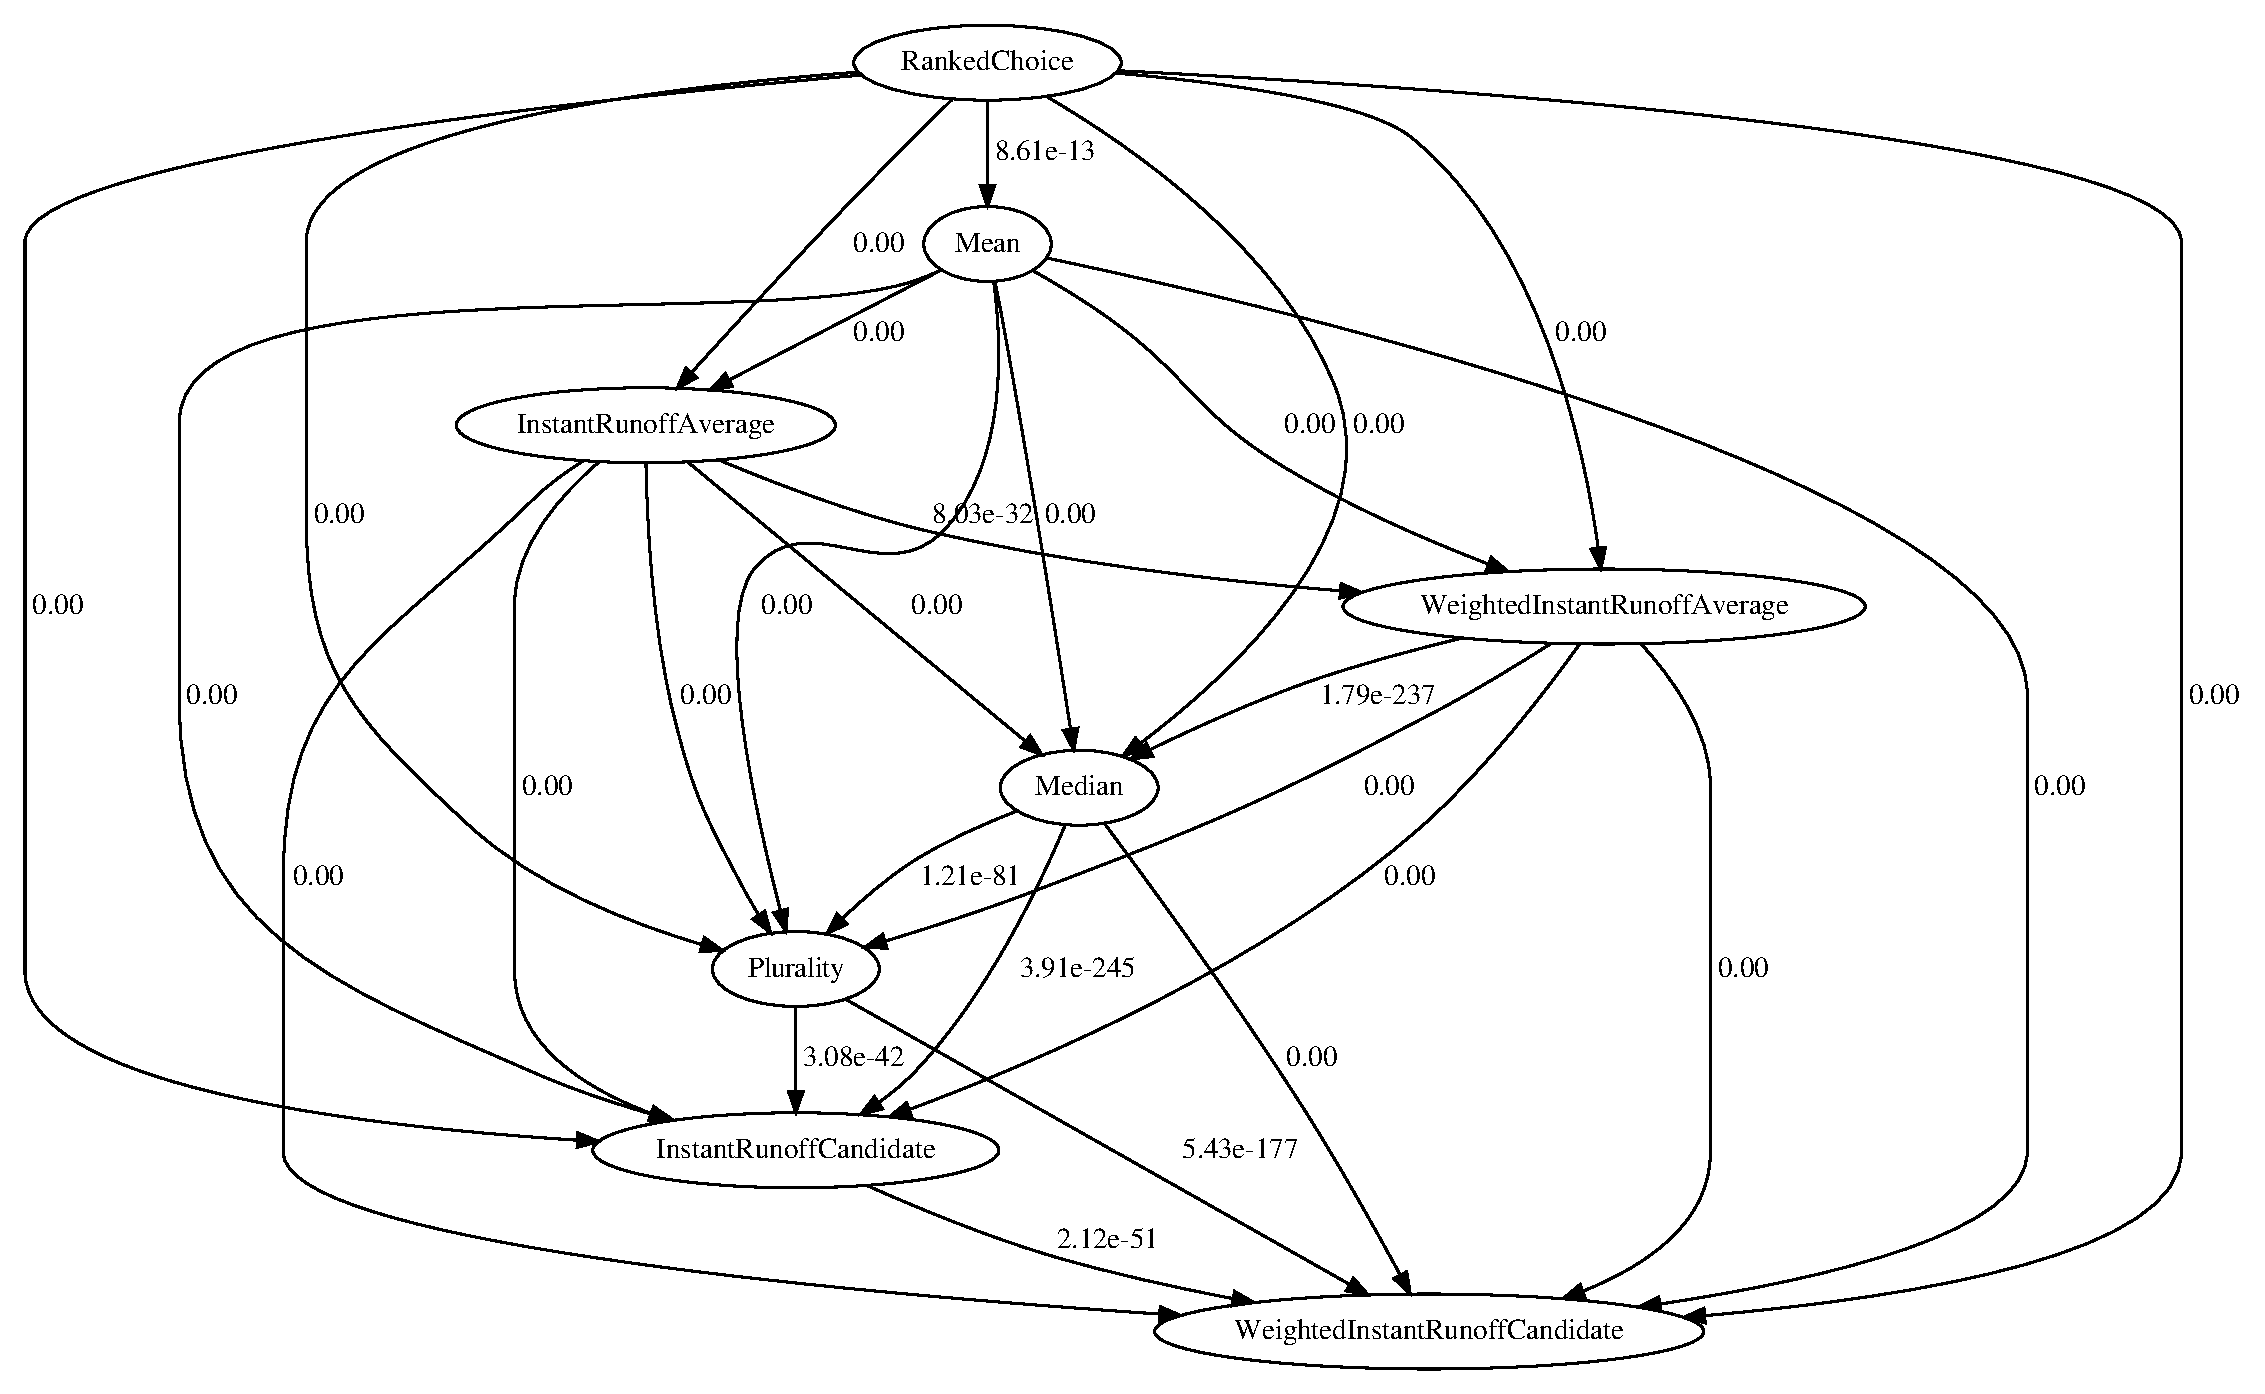
\includegraphics[
        angle=90,
        width=\textwidth,
        height=\dimexpr
        \textheight - 4 % Could also be .9\textheight
        \baselineskip,
        keepaspectratio]
    {./content/figures/voting_mechanisms/all-voting-mechanisms-p-values.gv}
    \caption{The p-values for all voting mechanisms, given the alternative is one
    population is lesser than the other.
    An arrow pointing to another voting mechanism indicates the `from' mechanism beats
    the `to' mechanism.}
    \label{fig:all-voting-mechanisms-p-values}
\end{figure}


\appendixsection{Distributions of Variables}
The distribution of variables for each voting mechanism is displayed as a
KDE graph in the figures of this section.

\begin{figure}[!t]
    \centering
    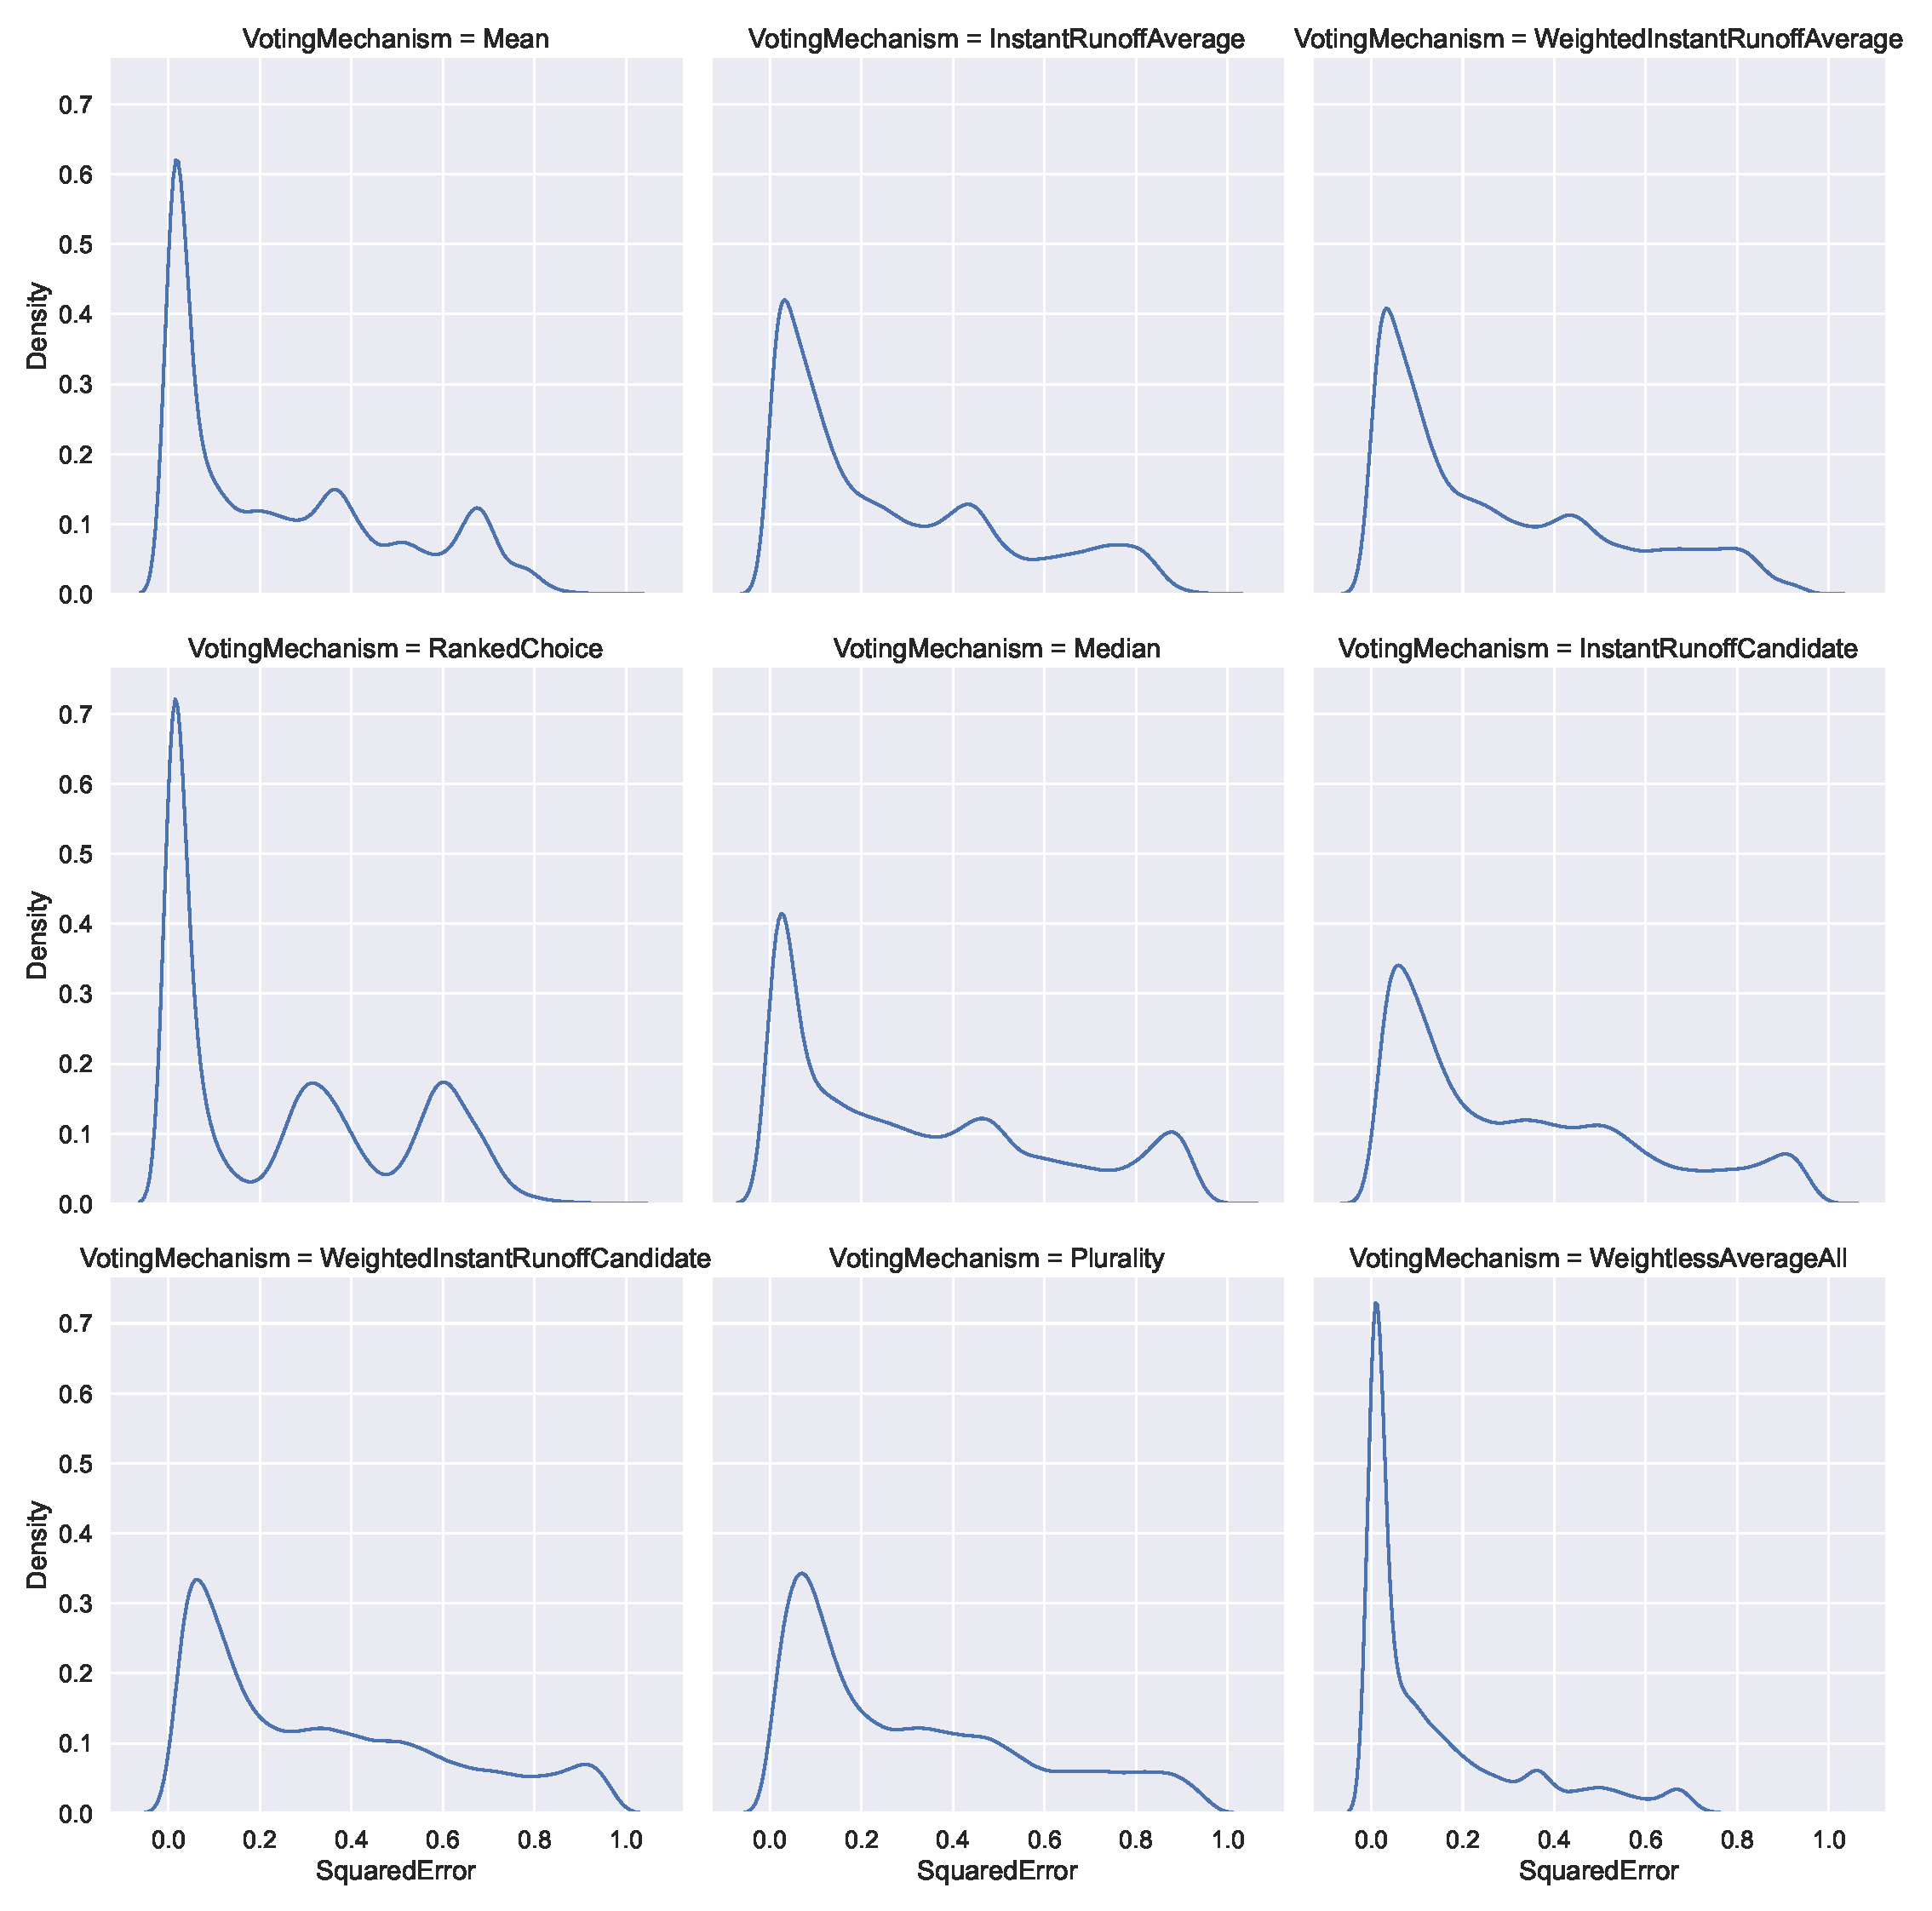
\includegraphics[
        width=\textwidth,
        height=\dimexpr
        \textheight - 2 % Could also be .9\textheight
        \baselineskip,
        keepaspectratio]
    {./content/figures/voting_mechanisms/voting_mechanisms_error_distribution}
    \caption{The distribution of squared error by voting mechanism.}
    \label{fig:voting_mechanisms_error_distribution}
\end{figure}

\begin{figure}[!t]
    \centering
    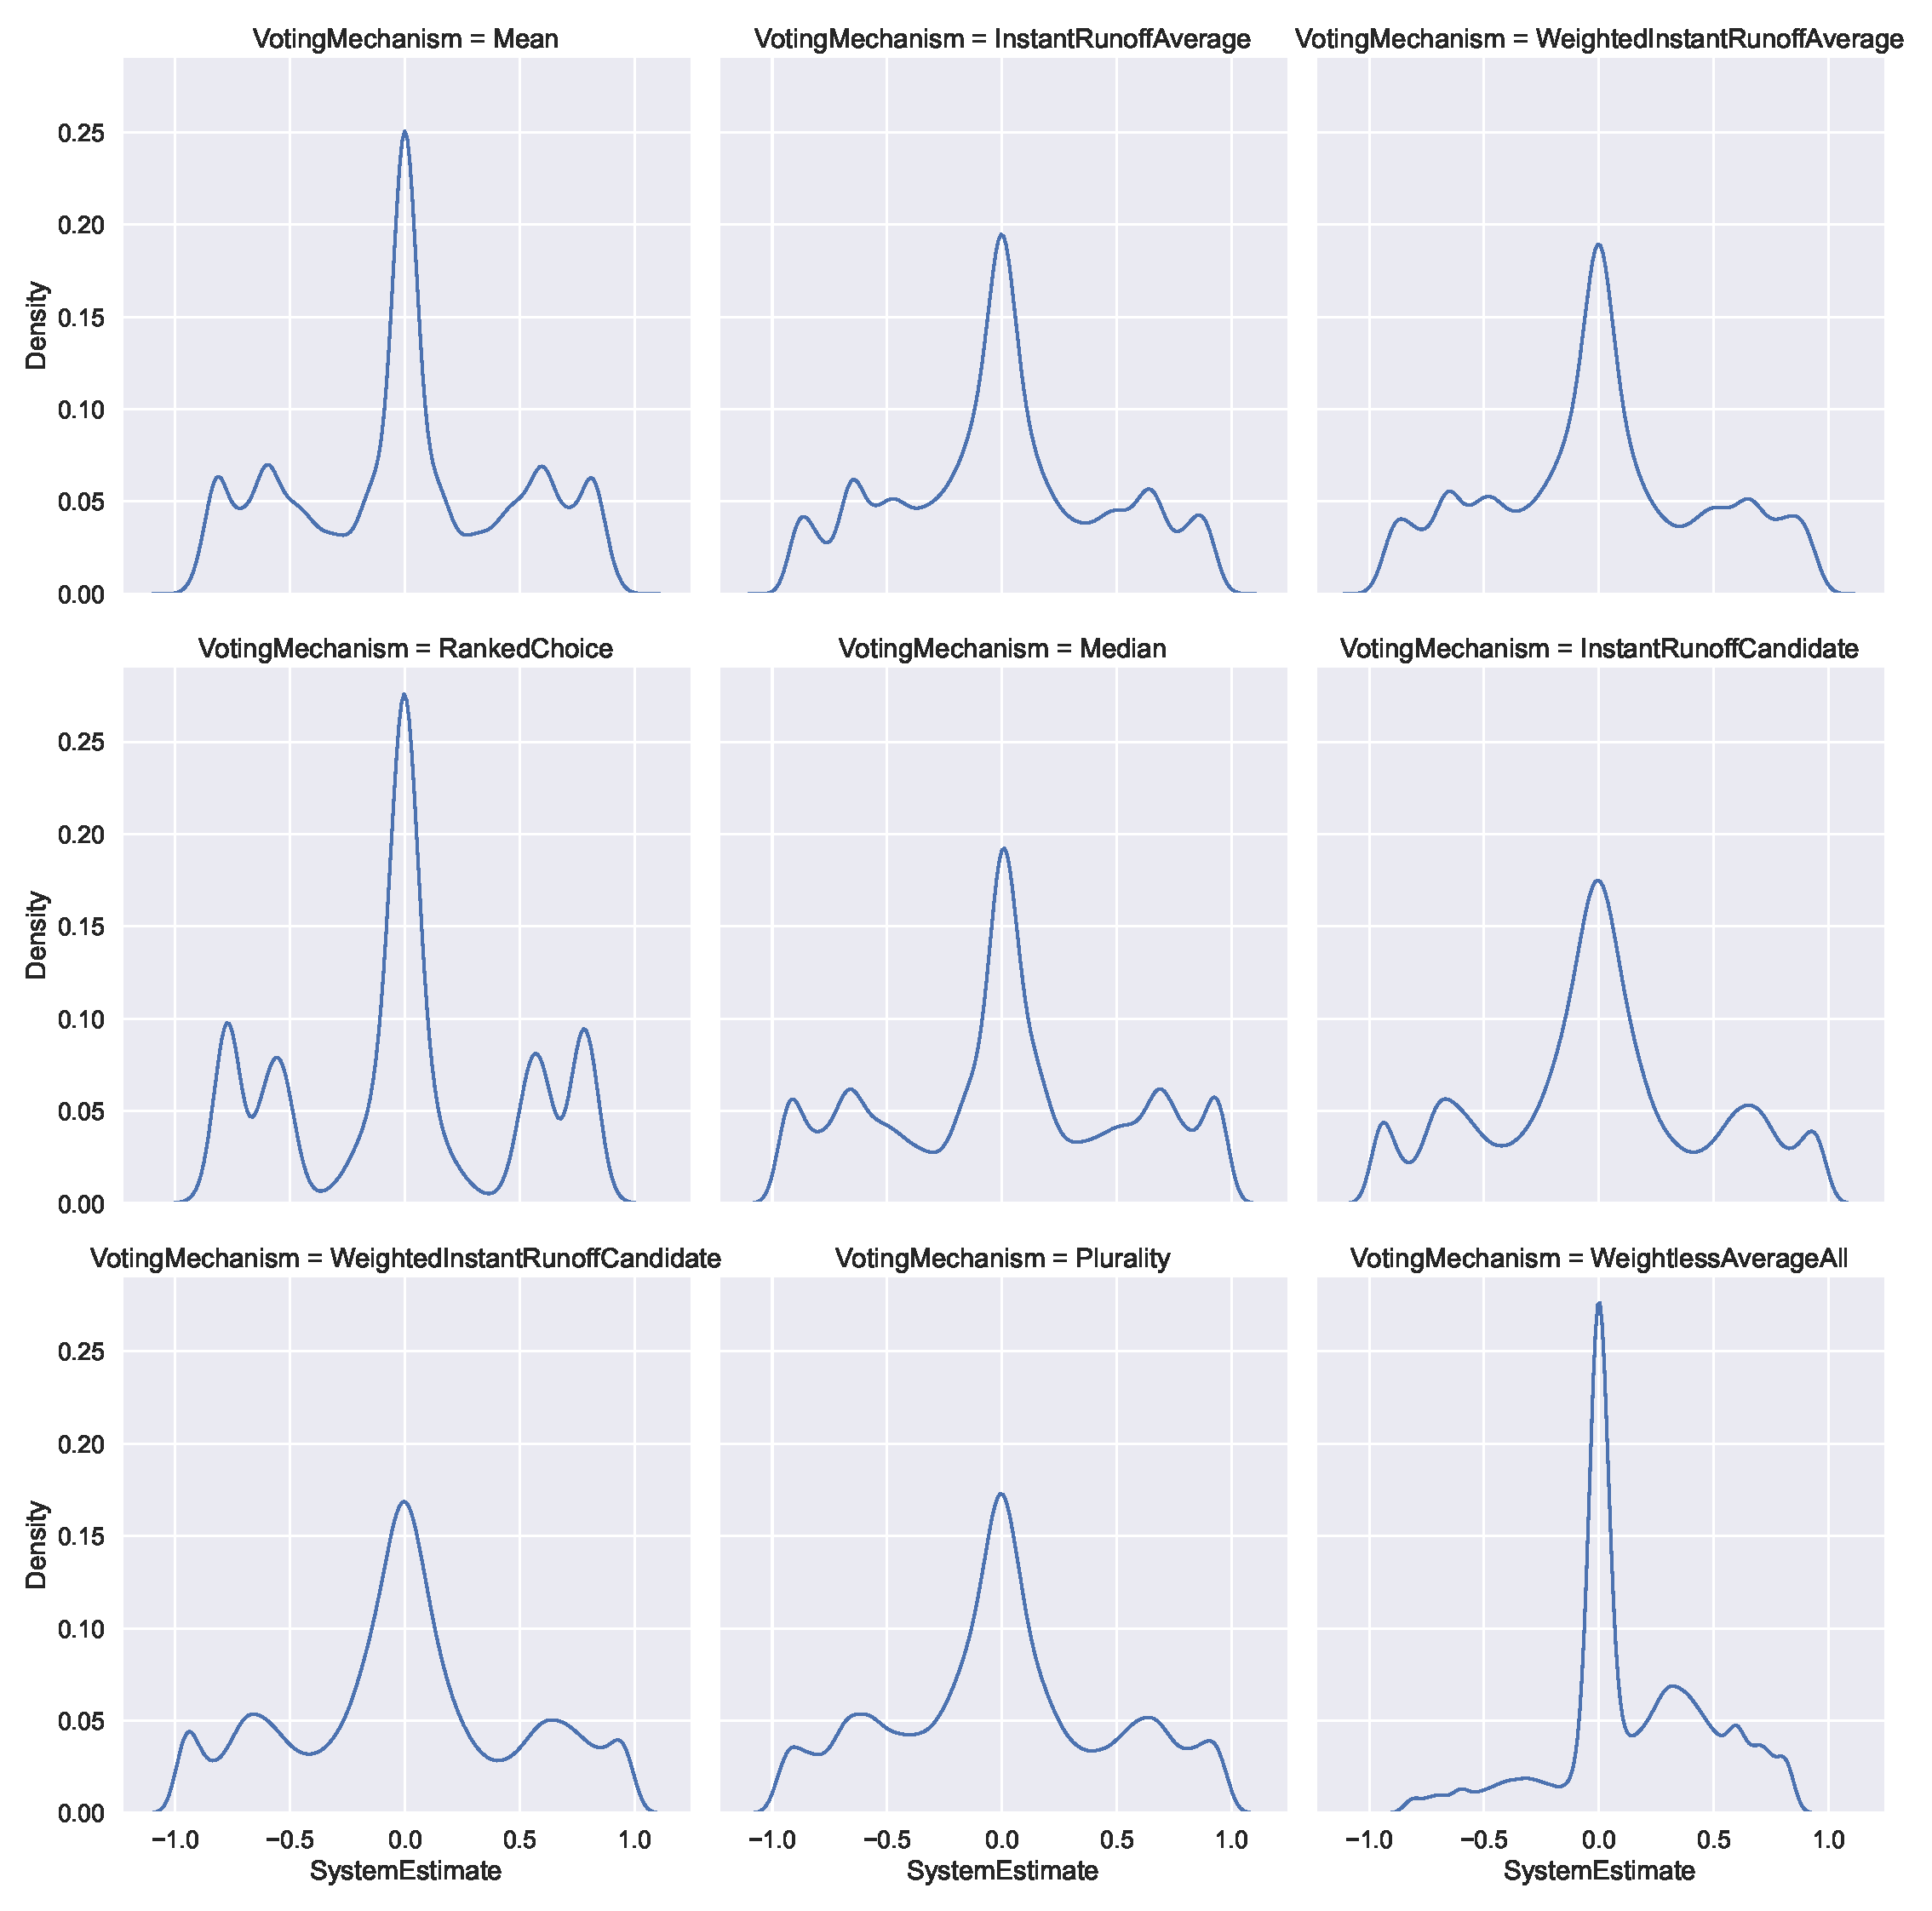
\includegraphics[
        width=\textwidth,
        height=\dimexpr
        \textheight - 2 % Could also be .9\textheight
        \baselineskip,
        keepaspectratio]
    {./content/figures/voting_mechanisms/voting_mechanisms_estimate_distribution}
    \caption{The distribution of system estimate by voting mechanism.}
    \label{fig:voting_mechanisms_estimate_distribution}
\end{figure}

\appendix{Visualizations}\label{chap:visualizations}
\begin{figure}[htbp]
    \centering
    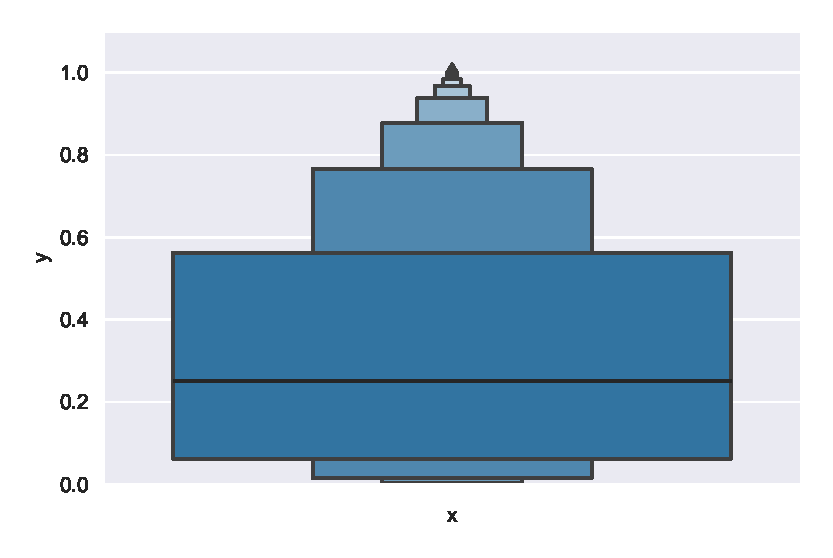
\includegraphics[scale=0.5]
    {./content/figures/expected_even_distribution_squared_error}
    \caption{Expected squared error distribution given a uniform distribution
    of estimates.}
    \label{fig:expected_even_distribution_squared_error}
\end{figure}

\begin{figure}[htbp]
    \centering
    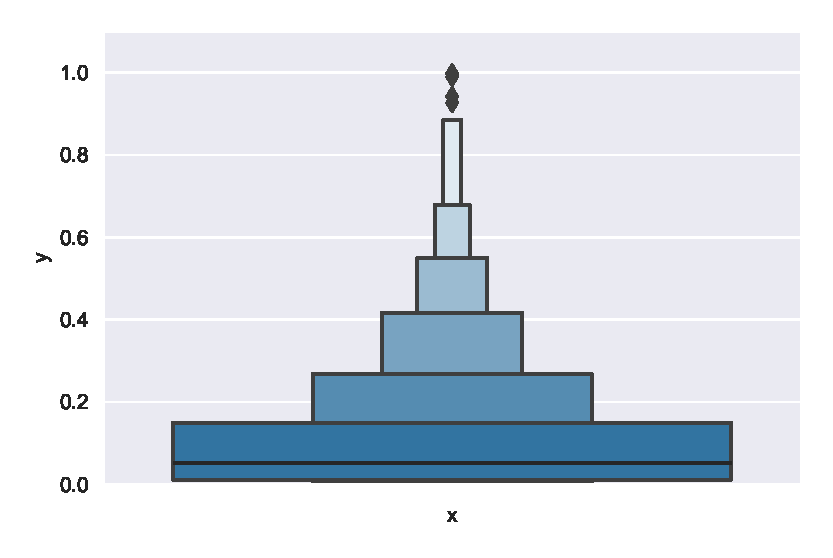
\includegraphics[scale=0.5]
    {./content/figures/expected_gaussian_distribution_squared_error}
    \caption{Expected squared error distribution given a gaussian distribution
    of estimates.}
    \label{fig:expected_gaussian_distribution_squared_error}
\end{figure}

    %
% This is an example of a vita page.  
% Format is not tightly specified. This example comes from Lili Ma.
%
%  Time-stamp: "[vita.tex] last modified by Scott Budge (scott) on 2012-07-16 (Monday, 16 July 2012) at 11:18:06 on goga"
%
%  Info: $Id$   USU
%  Revision: $Rev$
% $LastChangedDate$
% $LastChangedBy$
%

\begin{vita}

\begin{center}
{\Large \bf Michael D. Hegerhorst}\\
\end{center}

\section*{Published Journal Articles}
    \begin{itemize}
    \item Rational Radial Distortion Models of Camera Lenses with Analytical Solution for Distortion Correction, Lili
    Ma, YangQuan Chen, and Kevin L. Moore, {\it International Journal of Information Acquisition}, {\it Accepted}.

    \item A Small Mobile Robot for Security and Inspection Operations, N.S. Flann, K. L. Moore, and Lili Ma, {\it Control Engineering Practice}, vol. 10, pp. 1265-1270,
    2002.
    \end{itemize}

\section*{Published Conference Papers}
    \begin{itemize}
    \item Range Identification for Perspective Dynamic Systems Using
      Linear Approximation, Lili Ma, YangQuan Chen, and Kevin
      L. Moore, in {\it Proc. IEEE Int. Conf. on Robotics and
        Automation (ICRA)},
    2004.
  \item Range Identification for Perspective Dynamic System with
    Single Homogeneous Observation, Lili Ma, YangQuan Chen, and Kevin
    L. Moore, in {\it Proc. IEEE Int. Conf. on Robotics and Automation (ICRA)},
    2004.
  \item Blind Detection and Compensation of Camera Lens Geometrical
    Distortions, Lili Ma and YangQuan Chen, {\it SIAM Imaging
      Science}, 2004.
  \item Flexible Camera Calibration Using a New Analytical Radial
    Undistortion Formula with Application to Mobile Robot
    Localization, Lili Ma, YangQuan Chen, and Kevin L. Moore, in {\it
      Proc. Int. Symposium on Intelligent Control (ISIC)}, 2003.
  \item Sonar and Laser Based HIMM Map Building for Collision
    Avoidance for Mobile Robots, Lili Ma and Kevin L. Moore, in {\it
      Proc. International Symposium on Intelligent Control (ISIC)},
    2003.
  \item Wireless Visual Servoing for ODIS - An Under Car Inspection
    Mobile Robot, Lili Ma, Matthew Berkemeier, YangQuan Chen, Morgan
    Davidson, Vikas Bahl, and Kevin L. Moore, in {\it Proc. IFAC World
      Congress}, Spain, July, 2002.
  \item Visual Servoing of an Omni-Directional Mobile Robot for
    Alignment with Parking Lot Lines, Matthew Berkemeier, Morgan
    Davidson, Vikas Bahl, YangQuan Chen, and Lili Ma, in {\it Proc.
      IEEE Int.  Conf. on Robotics and Automation (ICRA)}, May 2002.
  \item Some Sensing and Perception Techniques for an Omnidirectional
    Ground Vehicle with a Laser Scanner, Zhen Song, YangQuan Chen,
    Lili Ma, and You Chung Chung, in {\it Proc. IEEE Int. Symposium on
      Intelligent Control (ISIC)}, October 2002.
  \item A Small Mobile Robot For Security and Inspection Operations,
    Flann NS, Moore KL, and Ma L, in {\it Proc. IFAC Conference on Telematics
      Applications in Automation and Robotics}, July 2001.
    \end{itemize}

\end{vita}

    %}}}
\end{document}
